\section{Introduction}\label{sec:introduction}

Single-particle cryo-electron microscopy (cryo-EM) has revolutionized the field of structural biology over the last decades~\cite{dubochet1988cryo, frank2006three, chap0-nat2015MethodYear}.
The use of electron beams to image ice-embedded samples has permitted the recovery of 3D bio-structures at unprecedented resolution.
This ``resolution revolution'' has had a tremendous impact in biomedical research, providing invaluable insights into the biological processes that underlie many current diseases.

In single-particle cryo-EM, every 3D particle adopts a random orientation $\bth_i$ in the ice layer before being imaged with parallel beams of electrons.
Hence, the projection geometry associated to each acquired 2D projection (\figref{imaging-geometry}) is unknown.
Yet, this knowledge is essential for the tomographic reconstruction of bio-structures~\cite{Natterer2001mathematics}.
We consider that a cryo-EM measurement (\ie, a projection) $\p_i \in \R^{n_p}$ is acquired through
\begin{equation}
    \label{eqn:imaging-model}
    \p_i = \mathbf{C}_{\boldsymbol\varphi} \mathbf{S}_{\mathbf{t}_i} \mathbf{P}_{\bth_i} \x + \mathbf{n},
\end{equation}
where $\x \in \R^{n_x}$ is the unknown 3D density map~\cite{dimaio_creating_2007} (Coulomb potential).
%\mdeff{Alternative notation: $\p_i = \mathbf{C}(\boldsymbol\varphi) \mathbf{S}(\mathbf{t}) \mathbf{P}(\bth_i) \x + \mathbf{n}$ if we want to write $\mathbf{R}(\bth_i) = \mathbf{R}(q_i) = \mathbf{R}(-q_i)$ later.}
%\mdeff{Alternative notation: $\x: \R^3 \rightarrow \R$ and $\p_i: \R^2 \rightarrow \R$ as functions, so $\x$ can be rotated by $\mathbf{R} \in \mathbf{SO}(3)$ as $\mathbf{R}\x$. But then $\x$ is not a vector for the SiameseNN.}
The operator $\mathbf{P}_{\bth_i}: \R^{n_x} \to \R^{n_p}$ is the projection along the orientation $\bth_i$ (\ie, the x-ray transform).
% consistency: 3D pose = orientation
The operator $\mathbf{S}_{\mathbf{t}_i}: \R^{n_p} \to \R^{n_p}$ is a shift of the projection by $\mathbf{t}_i = (t_{i_1}, t_{i_2})$.
The convolution operator $\mathbf{C}_{\boldsymbol\varphi}: \R^{n_p} \to \R^{n_p}$ models the microscope point-spread function (PSF) with parameters $\boldsymbol\varphi = (d_1, d_2, \alpha_\mathrm{ast})$, where $d_1$ is the defocus-major, $d_2$ is the defocus-minor, and $\alpha_\mathrm{ast}$ is the angle of astigmatism~\cite{vulovic_image_2013,rullgard_simulation_2011}.
Finally, $\mathbf{n} \in \R^{n_p}$ represents additive noise.
\figref{different-projections} illustrates the effect of projection, shift, and noise.
The challenge is then to reconstruct $\x$ from a set of projections $\{\p_i\}_{i=1}^P$ acquired along unknown orientations.
%\mdeff{We shall decompose $\mathbf{P}_{\bth_i}$ into a rotation $R(\bth_i)$ and an integration.} \lau{The most straightforward way is to simply rewrite $P_theta$ as a rotation operator, followed by a summation operator along lines. That being said, now that I look at it, I would suggest not to rewrite it like this; this is really not so standard in the cryo-EM community. Plus everyone now that the rotation operator is implicitly contained in the projection one, so it's not really needed either.}

% \tdplotsetmaincoords{60}{110}
% \pgfmathsetmacro{\rvec}{.8}
% \pgfmathsetmacro{\thetavec}{30}
% \pgfmathsetmacro{\phivec}{60}
% \begin{figure}
% \centering
% \begin{tikzpicture}[scale=4,tdplot_main_coords]
%     \coordinate (O) at (0,0,0);
%     \draw[thick,->] (0,0,0) -- (1,0,0) node[anchor=north east]{$\bsx_1$};
%     \draw[thick,->] (0,0,0) -- (0,1,0) node[anchor=north west]{$\bsx_2$};
%     \draw[thick,->] (0,0,0) -- (0,0,1) node[anchor=south]{$\bsx_3$};
%     \tdplotsetcoord{P}{\rvec}{\thetavec}{\phivec}
%     \draw[-stealth,very thick,color=red] (O) -- (P);
%     \draw[dashed, color=red] (O) -- (Pxy);
%     \draw[dashed, color=red] (P) -- (Pxy);
%     \tdplotdrawarc{(O)}{0.2}{0}{\phivec}{anchor=north}{$\theta_1$}
%     \tdplotsetthetaplanecoords{\phivec}
%     \tdplotdrawarc[tdplot_rotated_coords]{(0,0,0)}{0.5}{0}%
%         {\thetavec}{anchor=south west}{$\theta_2$}
%     \draw[dashed,tdplot_rotated_coords] (\rvec,0,0) arc (0:90:\rvec);
%     \draw[dashed] (\rvec,0,0) arc (0:90:\rvec);
%     \tdplotsetrotatedcoords{\phivec}{\thetavec}{0}
%     \tdplotsetrotatedcoordsorigin{(P)}
%     \draw[dashed,blue,tdplot_rotated_coords,-] (-.4,0,0)
%         -- (.4,0,0) node[anchor=north west]{};
%     \draw[dashed,blue,tdplot_rotated_coords,-] (0,-.4,0)
%         -- (0,.4,0) node[anchor=west]{};
%     \draw[blue,tdplot_rotated_coords,-]  (-.4,.4,0) -- (.4,.4,0)  -- (.4,-.4,0) -- (-.4,-.4,0) -- (-.4,.4,0)   node[anchor=north]{};
%     \tdplotdrawarc[tdplot_rotated_coords]{(0,0,0)}{0.2}{0}%
%         {30}{anchor=north west,color=black}{$\theta_3$}
%     \tdplotsetrotatedcoords{\phivec}{\thetavec}{30}
%     \draw[thick,tdplot_rotated_coords,->] (0,0,0)
%         -- (.3,0,0) node[anchor=north west]{$\bsy_1$};
%     \draw[thick,tdplot_rotated_coords,->] (0,0,0)
%         -- (0,.3,0) node[anchor=west]{$\bsy_2$};
%     \node[blue] at (0.4,0.45,1.2) {$\Omega_{\mathrm{2D}}$};
%     \node[red] at (1.5,0.75,1.2) {$\bvth_{\bth}$};
%     \tdplotsetrotatedthetaplanecoords{45}
% \end{tikzpicture}
% \caption*{\mdeff{Kept as reference for \figref{imaging-geometry} as this tikz figure is beautiful. Will be commented out in the end.}}
% \end{figure}

\begin{figure}
    \begin{minipage}[t]{0.48\linewidth}
        \centering
        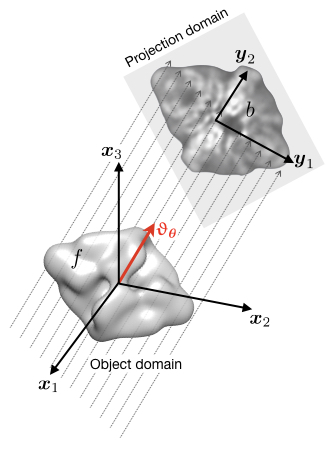
\includegraphics[height=0.7\linewidth]{geomProj3D}
        \caption{%
            % * (i) what we mean by a projection and an orientation (the two most important objects of our paper), and
            % * (ii) how a projection (=integration through z in the new coordinate system) is made from a 3D volume.
            % $\p_i = \mathbf{P} \Rot(\bth) \x$ \todo{($\mathbf{P}$ is a projection/integration)}.
            Geometry of the imaging model defined in \eqnref{imaging-model}.
            The 3D density $\x$ in the coordinate system $(x_1, x_2, x_3)$ is imaged along the \textit{orientation} $\bth$ to produce the 2D \textit{projection} $\p$ in the coordinate system $(y_1, y_2)$ of the microscope's detector plane.
            The orientation $\bth = (\theta_3, \theta_2, \theta_1)$ is decomposed as the direction $(\theta_2, \theta_1) \in [0,\pi] \times [0,2\pi[$ (parameterizing the sphere $\mathbb{S}^2$) and the in-plane rotation $\theta_3 \in [0,2\pi[$ (parameterizing the circle $\mathbb{S}^1$).
            In our work, we represent the orientation $\bth$ as a unit quaternion $q$.
            %The 3D rotation $\Rot(\bth) = \Rot(q) \in \SO(3)$ maps the object coordinate system to the projection coordinate system.
            %\mdeff{$\Rot$, $\bth$, and $q$ all represent orientations. That's the problem with notation that separates the representation not the semantic (though we might need that separation later).}
        }\label{fig:imaging-geometry}
    \end{minipage}
    \hfill
    \begin{minipage}[t]{0.48\linewidth}
        \centering
        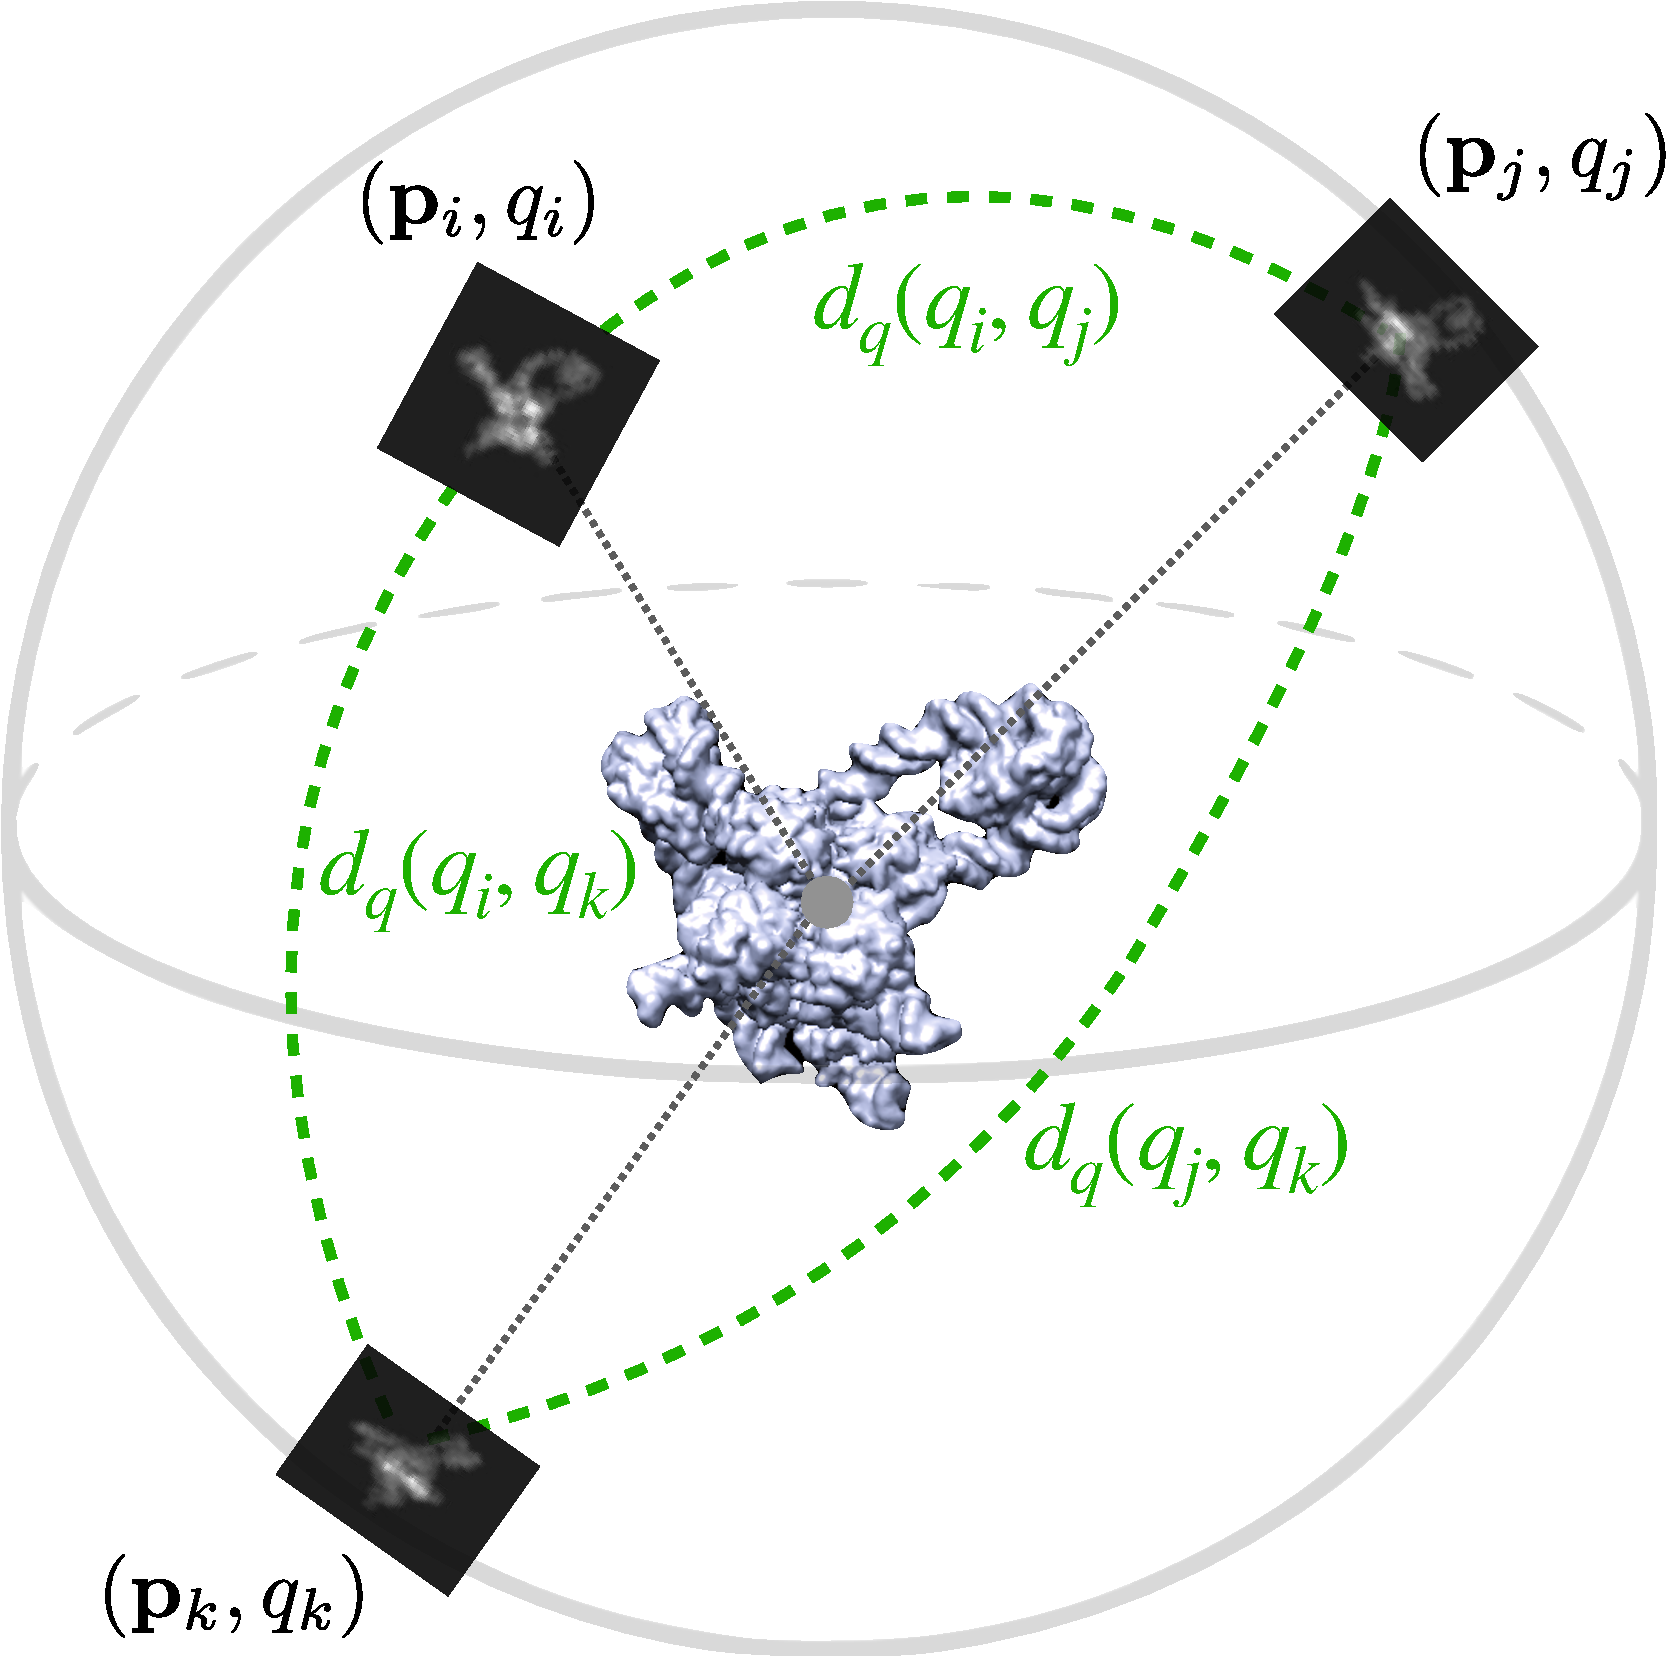
\includegraphics[height=0.7\linewidth]{intuition-method}
        \caption{%
            Single-particle cryo-EM produces $P$ projections (with $P$ in the order of $10^5$) from unknown orientations: $\{(\p_i, q_i)\}_{i=1}^P$.
            Observing that distances between orientations constrain the latter, we aim to \textit{recover the orientations} $\{q_i\}$ from $\{d_q(q_i, q_j)\}$, where $d_q(q_i, q_j)$ is the distance (angle) between orientations $q_i$ and $q_j$.
            Observing that the similarity between projections depends on their relative orientation, we aim to \textit{estimate the distance} $d_q(q_i, q_j)$ from the projections $(\p_i, \p_j)$.
            % \todo{The projections don't look to be on the surface of the sphere: They should be on tangent planes.}
            % \todo{The gray line to the center is the projection direction to be labeled $(\theta_1, \theta_2)$ with a color consistent with \figref{imaging-geometry}.}
            % \todo{The two green arcs seems too much like a single one.}
        }\label{fig:intuition-method}
    \end{minipage}
\end{figure}

% RELATED WORKS

A popular approach is to alternatively refine the 3D structure and an estimation of the orientations~\cite{penczek1994ribosome,Baker1996,Dempster1977,sigworth1998maximum,scheres2012bayesian,zehni2020joint}.
Yet, the outcome of these iterative-refinement procedures is still often predicated on the quality of the initial reconstruction, or, equivalently, on the initial estimation of the orientations~\cite{sorzano2006optimization,henderson2012outcome}.

Several methods have been designed to produce a first rough \textit{ab initio} structure for the refinement procedure~\cite{singer2020computational}.
An early approach~\cite{kam1980reconstruction} proposed to reconstruct an initial structure such that the first few moments of the distribution of its theoretical measurements match the ones of its experimental projections.
Since then, \textit{moment-matching} techniques have been refined and extended~\cite{salzman1990method,goncharov1988integral,sharon2019method}, \eg, to accommodate for non-uniform orientation configurations.
However, they typically remain sensitive to error in data and can require relatively high computational complexity.

Another popular approach relies on the central-slice theorem, which relates the Fourier transform of a projection to a plane (orthogonal to the projection direction) in the Fourier transform of the 3D object~\cite{Natterer2001mathematics}.
Hence, every two projections \textit{de facto} share a common 1D intersection in the 3D Fourier domain, and three projections theoretically suffice to define a coordinate system from which their orientations can be deduced~\cite{van1987angular}.
Exploiting this principle, \textit{common-lines} methods aim at uniquely determining the orientations of each projection by identifying the common-lines between triplets of projections~\cite{penczek1994ribosome,mallick2006structure,singer2010detecting,wang2013orientation,greenberg2017common,pragier2019common}---a real technical challenge given the massive amount of noise in cryo-EM data.
%If needs be for downside: sensitivity to high-noise levels, small particles, etc.

Alternatively, the marginalized maximum likelihood (ML) formulation of the reconstruction problem~\cite{sigworth1998maximum}---classically used for the iterative-refinement procedures themselves---can be minimized using stochastic gradient descent~\cite{punjani2017cryosparc}.
This permits to avoid the need for an initial volume estimate, at the possible cost of greater convergence instability.
More recently, the recovery of geometrical information from unknown view tomography of 2D point sources has been proposed~\cite{zehni2019distance}, but the extension to 3D cryo-EM tomography is not straightforward.
Finally, \cite{miolane2019estimation} proposed to recover the in-plane rotations by learning to embed projections in an appropriate latent space, but only after directions had been estimated through three rounds of 2D classification in RELION\@.

Despite the many aforementioned advances, the task of providing a robust initial volume remains a notoriously arduous challenge in single-particle cryo-EM due to the high-dimensionality and strong ill-posedness of the underlying optimization problem.
%\mdeff{How is our method different from previous work? What's its singularity? Why do we expect it to solve the aforementioned issues? This isn't a survey: The related work is here to build a stage for our work to stand on.}
On the other hand, deep learning has had a profound influence in imaging in reason of the remarkable ability of convolutional neural networks to capture relevant representations of images~\cite{lecun2015deep}.

In this work, we present a new learning-based approach to recover the unknown orientations directly from the acquired set of projections.
%, hence bypassing some of the aforementioned limitations.
% \mdeff{That's method:} The novelty consists in first estimating the relative distances between pairs of projections (by using a Siamese neural network previously trained on a synthetic dataset), and then recovering the absolute orientation of each projections from these relative distances.
By doing so, orientations are recovered without the need for any intermediate reconstruction procedure or initial volume estimate. %, which has useful implications for SPA\@.
%\mdeff{``bypassing some limitations'' and ``has useful implications'' are too vague IMO\@. Could we be more specific? Not on the how (that's the method) but on the why. Think about an ML audience.}
%\mdeff{Idea: Our method is direct (as opposed to iterative refinement schemes) and does not require any prior model of the reconstructed protein.}
%Our two-step method  learns to estimate the unknown orientation $\bth_i$ (represented by a unit quaternion $q_i$) associated to each projection $\p_i$ in a single-particle cryo-EM dataset without relying on any intermediate reconstruction procedure.

%\mdeff{Content. (p1) Why is the general problem of protein reconstruction important and difficult. (p2) Short background on single-particle cryo-EM and how reconstruction is done. (p3) Previous work on orientation estimation (or initial structure estimation). If there's none (because people have researched other routes), state it and write why it's an interesting route to explore. How does it compare to initial rough structure estimation? Or whatever the other routes are. (p4) Our contribution on top of previous work.}
